\chapter{Test}
The primary test purpose is to reveal the presence of faults. The main idea behind testing consists in applying test data to inputs of the IC, design, wafer, dice, or any other system called Unit Under Test (UUT). The test data applied to the inputs is called the test vector or test stimuli and the data collected from the outputs - the response of the UUT. The term test pattern is used to describe the test vectors together with expected correct responses. A test set relates to a series of test patterns. After applying test vectors and capturing the responses, they are compared with a fault free response stored in the test pattern. If they differ in any position or value, fault is uncovered. The \autoref{fig:test} shows the typical test environment

\begin{figure}[H]
\centering
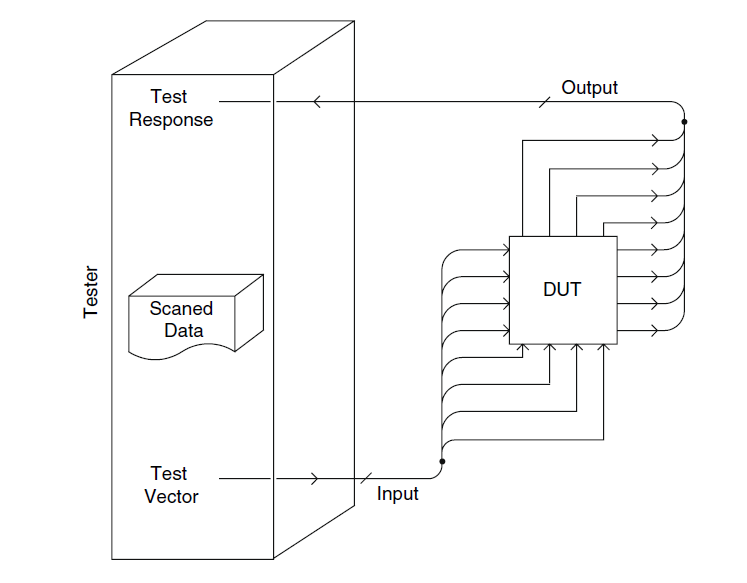
\includegraphics[width=0.65\textwidth]{figures/test.png}
\caption{The tester principle~\cite{book:Navabi}}
\label{fig:test}
\end{figure}


\section{Fault models}

While it is possible to prove the presence of faults in the design, there is no method proving their absence. The amount of different faults and their variety is countless, hence there are means needed to model how those faults affect the system. The fault itself is not visible to the tester itself (except from visual tests) and has to be stimulated to manifest, and in best case, propagete to the UUT outputs. Many different faults can have the same effect, so investigating the effects of faults may bring better results. The fault effects are called failure modes and they have to be modeled in order to conduct tests. Such fault models serve the purpose of altering the data flow, in the similar way, as the real faults would. It allows to develop test vectors to stimulate and propagate the real faults effects. There are two groups of fault models. The ones that describe faults affecting the logical operations and ones describing the defects in parameters. The most common logical fault models are:
\begin{itemize}
    \item Stuck-At-Fault consists in an assumption that node in the design has a permanent value and doesn't respond to the logical transitions forced on it. The node can Stuck-at-0 (SA0) or Stuck-at-1 (SA1)
    \item Bridging fault assumes that two nodes interact with each other unintentionally producing either a Wired-AND effect with 0-dominant connection or Wired-OR effect being 1 dominant.
    \item Delay fault may be considered as a parametric fault rather than a logic fault but can be detected thanks to digital test vectors and rising the operational frequency until the test fails. 
    \item Memory fault (logical faults considered)
    \item Single Event Transient (SET) describes a glitch in combinational logic that travels trough design.
    \item Single Event Upset (SEU) describes the situation when the incorrect voltage level caused by SET gets stored in the memory or the memory state changes. Can affect more memory cells at once.
    \item Single Event Latchup (SEL) - a highly loaded particle makes a locked transistor conduct leading to short in CMOS logic. Requires a power reset and may lead to a hard fault, because of a very high temperature~\cite{report:altera}.
\end{itemize}
The logical faults The parametric faults are modeled through:
\begin{itemize}
    \item Bridging fault assumes resistive unintentional connection between two nodes
    \item Memory fault (non-logical faults considered)
    \item Open-circuit fault in interconnect metal
    \item Stuck-open and stuck-short faults in transistors
    \item $I_DDQ$ Fault - measuring the current by power supply during static operation of the design (while there is no switching activity)
\end{itemize}
All mentioned models represent failure modes in digital hardware logic, even the analog or mixed signal tests consider only digital cicuits. Some operations however take less time or energy when moved from digital domain to analog one~\cite{Prof Vierhaus Lectures}. In modern communication systems there is a rapid growth in analog and mixed circuitry that is also vulnerable to faults. The number of such faults is again countless and some failure mode representation is required. The continuous characteristic of analog systems allows only for two failure modes:
\begin{itemize}
    \item Catastrophic failures - the system is not functional at all
    \item Unacceptable performance - the service is still provided but some of the functionality lies outside of the acceptable range of the specification
\end{itemize}
The distinction between them lies only in the definition of catastrophic failure and definition range of the system. On higher abstraction levels the catastrophic fault may only be considered as a parametric one~\cite{book:Kabisatpathy}, following the rule of fault propagation mentioned in~\autoref{fig:propagation}.




%diagnostic test
%online offline testing
% DFT, scan path, boundry scna, BIST
